\chapter{Nonlinear Conjugate Gradient Methods}

\section{Introduction}

\textbf{Idea:} Adapt the linear conjugate gradient (efficient for quadratic problems) to general nonlinear objective functions.

\section{Fletcher-Reeves Method}

Fletcher and Reeves \cite{fletcher1964function} proposed two major changes compared to the linear algorithm to minimize any function $f$.

\subsection{1. Line Search}
Unlike the quadratic case where the step $\alpha_k$ is given by an exact formula, here we substitute the formula:
\[
\alpha_k = \frac{r_k^\top r_k}{p_k^\top A p_k}
\]
with a \textbf{line search} to approximate the minimum of $f$ along the direction $p_k$.

\subsection{2. Substituting the residual with the gradient}
In the linear case, the residual $r_k$ corresponded to the gradient of the quadratic function $\phi$. For the general case, we substitute the gradient of $\phi$ with the gradient of $f$:
\[
r_k = \nabla \phi(x_k) \longrightarrow \nabla f_k.
\]

\subsection{Formula for \texorpdfstring{$\beta_{FR}$}{beta\_FR}}
The formula for $\beta$ used in the linear case ($\beta = \frac{r_{k+1}^\top r_{k+1}}{r_k^\top r_k}$) becomes the Fletcher-Reeves formula:
\[
\boxed{\beta_{FR} = \frac{\nabla f_{k+1}^\top \nabla f_{k+1}}{\nabla f_k^\top \nabla f_k}}.
\]
This defines Algorithm 9.

\begin{remarque}
There is no minus sign in this formula.
\end{remarque}

\begin{figure}[H]
\centering
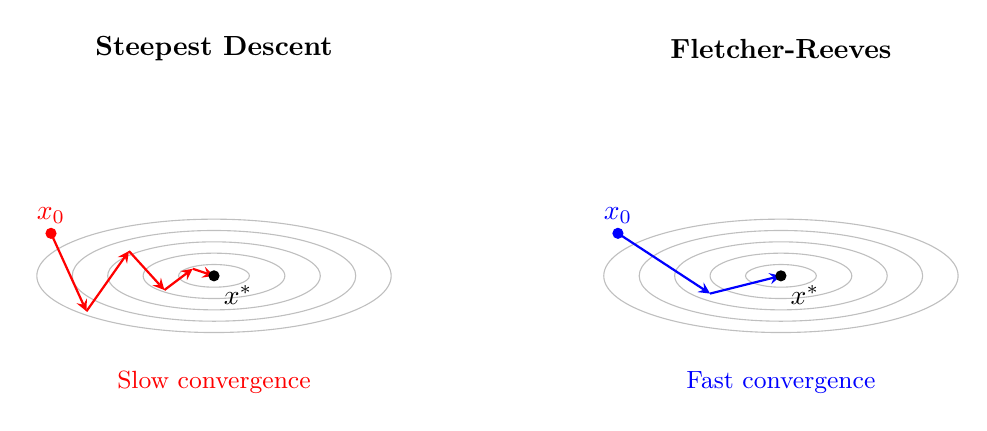
\begin{tikzpicture}[scale=0.9]
    % Left plot: Steepest Descent (zigzag)
    \begin{scope}[shift={(-4,0)}]
        \node at (0, 3.2) {\textbf{Steepest Descent}};
        
        % Draw elliptical contours
        \draw[gray!50] (0,0) ellipse (2.5cm and 0.8cm);
        \draw[gray!50] (0,0) ellipse (2.0cm and 0.64cm);
        \draw[gray!50] (0,0) ellipse (1.5cm and 0.48cm);
        \draw[gray!50] (0,0) ellipse (1.0cm and 0.32cm);
        \draw[gray!50] (0,0) ellipse (0.5cm and 0.16cm);
        
        % Steepest descent path (zigzag)
        \coordinate (sd0) at (-2.3, 0.6);
        \coordinate (sd1) at (-1.8, -0.5);
        \coordinate (sd2) at (-1.2, 0.35);
        \coordinate (sd3) at (-0.7, -0.2);
        \coordinate (sd4) at (-0.3, 0.1);
        \coordinate (sd5) at (0, 0);
        
        \draw[red, thick, -stealth] (sd0) -- (sd1);
        \draw[red, thick, -stealth] (sd1) -- (sd2);
        \draw[red, thick, -stealth] (sd2) -- (sd3);
        \draw[red, thick, -stealth] (sd3) -- (sd4);
        \draw[red, thick, -stealth] (sd4) -- (sd5);
        
        \filldraw[red] (sd0) circle (2pt) node[above] {$x_0$};
        \filldraw[black] (0,0) circle (2pt) node[below right] {$x^*$};
        
        \node[red] at (0, -1.5) {\small Slow convergence};
    \end{scope}
    
    % Right plot: Fletcher-Reeves (more direct)
    \begin{scope}[shift={(4,0)}]
        \node at (0, 3.2) {\textbf{Fletcher-Reeves}};
        
        % Draw elliptical contours
        \draw[gray!50] (0,0) ellipse (2.5cm and 0.8cm);
        \draw[gray!50] (0,0) ellipse (2.0cm and 0.64cm);
        \draw[gray!50] (0,0) ellipse (1.5cm and 0.48cm);
        \draw[gray!50] (0,0) ellipse (1.0cm and 0.32cm);
        \draw[gray!50] (0,0) ellipse (0.5cm and 0.16cm);
        
        % Fletcher-Reeves path (more direct, conjugate directions)
        \coordinate (fr0) at (-2.3, 0.6);
        \coordinate (fr1) at (-1.0, -0.25);
        \coordinate (fr2) at (0, 0);
        
        \draw[blue, thick, -stealth] (fr0) -- (fr1);
        \draw[blue, thick, -stealth] (fr1) -- (fr2);
        
        \filldraw[blue] (fr0) circle (2pt) node[above] {$x_0$};
        \filldraw[black] (0,0) circle (2pt) node[below right] {$x^*$};
        
        \node[blue] at (0, -1.5) {\small Fast convergence};
    \end{scope}
\end{tikzpicture}
\caption{Comparison of steepest descent (left) and Fletcher-Reeves (right) on elliptical level curves. The Fletcher-Reeves method uses conjugate directions to converge faster.}
\label{fig:fr-vs-sd}
\end{figure}

\begin{figureexplanation}
Figure~\ref{fig:fr-vs-sd} illustrates the advantage of the nonlinear conjugate gradient (Fletcher-Reeves) over steepest descent. On an ill-conditioned quadratic function (elongated ellipses), steepest descent zigzags by alternating between orthogonal directions, while Fletcher-Reeves exploits conjugate directions to reach the minimum in fewer iterations.
\end{figureexplanation}

\subsection{Illustration on the Rosenbrock Function}

The \textbf{Rosenbrock function} $f(x,y) = (1-x)^2 + 100(y-x^2)^2$ is a classic test case for optimization algorithms. It has a unique minimum at $(1,1)$ but presents a very narrow and strongly curved valley that makes convergence difficult.

\begin{figure}[H]
\centering

\includegraphics[width=0.85\textwidth]{1.png}
\caption{The Rosenbrock function $f(x,y) = (1-x)^2 + 100(y-x^2)^2$, having a unique minimum at $(1,1)$.}
\label{fig:rosenbrock-surface}
\end{figure}

\begin{figureexplanation}
\textbf{Key points to observe:}
\begin{itemize}
    \item \textbf{Shape of the surface:} The parabolic valley ("banana valley") is clearly visible. The global minimum $(1,1)$ is at the bottom of this narrow valley.
    \item \textbf{Logarithmic scale:} The vertical axis uses $\log(Z)$ to visualize the large variations of the function.
    \item \textbf{Optimization difficulty:} Reaching the bottom of the valley is easy, but making progress along the valley towards the minimum is difficult for many methods.
\end{itemize}
\end{figureexplanation}

\begin{figure}[H]
\centering

\includegraphics[width=0.7\textwidth]{5.png}
\caption{Iterations of the Fletcher-Reeves method (nonlinear conjugate gradient) on the level curves of the Rosenbrock function.}
\label{fig:fletcher-reeves-rosenbrock}
\end{figure}

\begin{figureexplanation}
\textbf{Key points to observe:}
\begin{itemize}
    \item \textbf{Efficient trajectory:} The method converges to the minimum $(1,1)$ by exploiting conjugate directions, without explicitly using the Hessian.
    \item \textbf{Trade-off:} Fletcher-Reeves offers faster convergence than gradient descent, while avoiding the cost of computing the Hessian (necessary for Newton).
    \item \textbf{Adaptation to the nonlinear case:} Although conjugate gradient theory is optimal for quadratic functions, the method remains effective on this strongly non-quadratic function.
\end{itemize}
\end{figureexplanation}

%%%%%%%%%%%%%%%%%%%%%%%%%%%%%%%%%%%%%%%%%%%%%%%%%%%%%%%%%%%%
\subsection{Global Descent Property}

Unlike the quadratic case, the direction $p_k$ generated by Fletcher-Reeves is not automatically a descent direction.

We have the relation:
\[
\nabla f_k^\top p_k = -\|\nabla f_k\|^2 + \beta_{FR} \nabla f_k^\top p_{k-1}.
\]
If the second term is large, the direction can go upward. To guarantee descent, strict conditions must be imposed on the line search.

\begin{lemme}[Descent Condition]
Suppose that the step $\alpha_k$ satisfies the \textbf{strong Wolfe conditions} with a parameter $0 < c_2 < \frac{1}{2}$.
Then, the direction $p_k$ is always a descent direction and satisfies the following bounds for all $k$:
\[
-\frac{1}{1-c_2} \le \frac{\nabla f_k^\top p_k}{\|\nabla f_k\|^2} \le \frac{2c_2 - 1}{1-c_2}.
\]
\end{lemme}

\begin{proof}
\textbf{Preliminary.} Consider the function $t(\xi) = \frac{2\xi - 1}{1 - \xi}$.
This function is increasing on $[0, \frac{1}{2}]$.
We have $t(0) = -1$ and $t(1/2) = 0$.
Since $0 < c_2 < 1/2$, we have:
\[
-1 < \frac{2c_2 - 1}{1 - c_2} < 0.
\]

\textbf{Initialization ($k=0$).}
We have $p_0 = -\nabla f_0$, so $\nabla f_0^\top p_0 = -\|\nabla f_0\|^2$.
The ratio is:
\[
\frac{\nabla f_0^\top p_0}{\|\nabla f_0\|^2} = -1.
\]
The inequality is satisfied because:
\[
-\frac{1}{1-c_2} \le -1 < \frac{2c_2 - 1}{1 - c_2} \quad \text{(verified because } c_2 < 1/2 \text{)}.
\]

\textbf{Induction step.} Suppose the result is true for $k$.
Let's compute the ratio for $k+1$:
\[
\frac{\nabla f_{k+1}^\top p_{k+1}}{\|\nabla f_{k+1}\|^2} 
= \frac{\nabla f_{k+1}^\top (-\nabla f_{k+1} + \beta_{k+1}^{FR} p_k)}{\|\nabla f_{k+1}\|^2}
= -1 + \beta_{k+1}^{FR} \frac{\nabla f_{k+1}^\top p_k}{\|\nabla f_{k+1}\|^2}.
\]
Using the definition of $\beta_{FR} = \frac{\|\nabla f_{k+1}\|^2}{\|\nabla f_k\|^2}$, we simplify to:
\[
\frac{\nabla f_{k+1}^\top p_{k+1}}{\|\nabla f_{k+1}\|^2} = -1 + \frac{\nabla f_{k+1}^\top p_k}{\|\nabla f_k\|^2}.
\]

The curvature condition (second strong Wolfe condition) requires:
\[
|\nabla f_{k+1}^\top p_k| \le c_2 |\nabla f_k^\top p_k|.
\]
Since $p_k$ is a descent direction (induction hypothesis), $\nabla f_k^\top p_k < 0$. Thus $|\nabla f_k^\top p_k| = -\nabla f_k^\top p_k$.
The inequality becomes:
\[
|\nabla f_{k+1}^\top p_k| \le -c_2 \nabla f_k^\top p_k.
\]
This implies:
\[
c_2 \nabla f_k^\top p_k \le \nabla f_{k+1}^\top p_k \le -c_2 \nabla f_k^\top p_k.
\]

Dividing by $\|\nabla f_k\|^2$ and adding $-1$, we obtain the bounds:
\[
-1 + c_2 \frac{\nabla f_k^\top p_k}{\|\nabla f_k\|^2} \le \frac{\nabla f_{k+1}^\top p_{k+1}}{\|\nabla f_{k+1}\|^2} \le -1 - c_2 \frac{\nabla f_k^\top p_k}{\|\nabla f_k\|^2}.
\]
Using the induction hypothesis on the right-hand term shows that the bounds are preserved for $k+1$.
\end{proof}

%%%%%%%%%%%%%%%%%%%%%%%%%%%%%%%%%%%%%%%%%%%%%%%%%%%%%%%%%%%%
\section{Polak-Ribière Method}

Another very popular variant, often considered more efficient in practice, is the Polak-Ribière (PR) method.

\subsection{Definition and Properties}

Polak and Ribière proposed the following formula for $\beta$:
\[
\boxed{\beta_{k+1}^{PR} = \frac{\nabla f_{k+1}^\top (\nabla f_{k+1} - \nabla f_k)}{\|\nabla f_k\|^2}}.
\]

\paragraph{Coincidence with FR.}
If the function $f$ is strictly quadratic, then successive gradients are orthogonal ($\nabla f_{k+1}^\top \nabla f_k = 0$). In this case, the subtraction term vanishes and:
\[
\beta_{k+1}^{PR} = \beta_{k+1}^{FR}.
\]
PR therefore coincides with FR and the linear conjugate gradient on quadratic problems.

\paragraph{Descent problem.}
However, unlike Fletcher-Reeves, even strong Wolfe conditions do not guarantee that the direction $p_k$ generated by Polak-Ribière is a descent direction.

\subsection{\texorpdfstring{$\beta^{PR+}$}{beta\_PR+} Variant}

To guarantee generating descent directions, one frequently uses the following modification:
\[
\beta_{k+1}^{PR+} = \max\left( \beta_{k+1}^{PR}, 0 \right).
\]
This amounts to resetting the direction to the steepest descent direction ($p_{k+1} = -\nabla f_{k+1}$) when $\beta_{k+1}^{PR}$ becomes negative.

\subsection{Practical Remarks and Convergence Rate}

\begin{itemize}
    \item \textbf{Performance:} In practice, the PR method is often better than FR for general nonlinear functions and when the line search is inexact.
    \item \textbf{Restart:} A common strategy is to "restart" the algorithm every $n$ iterations by taking a Steepest Descent step. Note that this descent step corresponds to the initialization of the conjugate gradient method.
    \item \textbf{Convergence Rate:} With appropriate restarts, an $n$-step quadratic convergence can be proven:
    \[
    \|x_{k+n} - x^\star\| = O\left( \|x_k - x^\star\|^2 \right).
    \]
\end{itemize}

%%%%%%%%%%%%%%%%%%%%%%%%%%%%%%%%%%%%%%%%%%%%%%%%%%%%%%%%%%%%
\section{Global Convergence Analysis}

Here we study the conditions under which the gradient descends to zero.

\subsection{Assumptions (Assumptions A)}
To establish convergence, we make the following assumptions on the function $f$ and the level set $\mathcal{L} = \{x \in \R^n \mid f(x) \le f(x_0)\}$:
\begin{enumerate}
    \item The level set $\mathcal{L}$ is bounded.
    \item $f$ is continuously differentiable and its gradient is Lipschitz continuous in a neighborhood of $\mathcal{L}$.
\end{enumerate}

\subsection{Al-Baali's Theorem}

This important result establishes the global convergence of the Fletcher-Reeves method under strong Wolfe conditions with a sufficiently small $c_2$ parameter.

\begin{theoreme}[Al-Baali]
Under assumptions A, if the Fletcher-Reeves algorithm is implemented with strong Wolfe conditions and parameters satisfying:
\[
0 < c_1 < c_2 < \frac{1}{2},
\]
then the sequence of gradients converges to zero in the following sense:
\[
\liminf_{k \to \infty} \|\nabla f_k\| = 0.
\]
\end{theoreme}

\bigskip
\begin{checkpoint}
\begin{itemize}
    \item \textbf{Adaptation:} How do we go from linear CG to nonlinear CG (replacing the residual with the gradient, $\alpha_k$ with Line Search)?
    \item \textbf{$\beta$ Formulas}: What is the difference between Fletcher-Reeves (FR) and Polak-Ribière (PR)? Which one is generally better in practice?
    \item \textbf{Restart:} Why do we "restart" the algorithm (steepest descent step) periodically?
    \item \textbf{Descent:} Does nonlinear CG always guarantee a descent direction? (No for PR without modification, yes for FR with Strong Wolfe).
\end{itemize}
\end{checkpoint}
